\section{Coordination}\label{coordination}
This section analyses the \textbf{messages exchanged among the entities composing the prototype architecture}. There are \textbf{three phases} in this coordination process:
\begin{enumerate}
    \item \textbf{Grid connection}
    \item \textbf{Recruitment}
    \item \textbf{P2P messaging}
\end{enumerate}

\subsection{Grid connection}
This phase \textbf{connects a Node} (whether used by the Mobile or the Desktop client) \textbf{or an Invoking Endpoint Prototype to the Broker Service using a Socket connection} through the Socket.io framework. \textbf{The Broker Service registers the connections and uses them in the Recruitment phase}.

\subsection{Recruitment}
The recruitment phase \textbf{connects a requestor device} (that becomes the Master in the P2Pconnection) \textbf{to an actual device that will perform a Contribution} (becoming the Slave). \textbf{While a Slave is necessarily a Node, a Master can either be an Invoking Endpoint or a Node}, allowing to obtain either an \textbf{Invoking Endpoint to Node connection} or a \textbf{Node to Node connection}.

This phase is \textbf{executed exchanging messages among the soon-to-be Peers using the previously established Socket connections, but ends with a direct P2P connection} between the Master and the Slave through the WebRTC framework.

\vspace{3mm}
\begin{figure}[!ht]
    \centering
    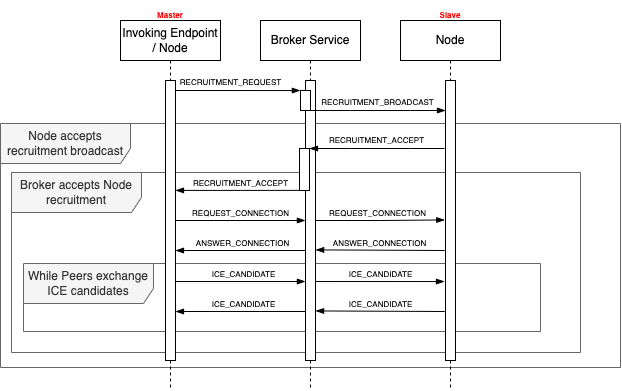
\includegraphics[scale=0.65]{document/chapters/chapter_6/images/recruitment_messages.png}
    \caption{Recruitment - Sequence Diagram}
    \label{fig:recruitment_messages}
\end{figure}

\textit{Figure \ref{fig:recruitment_messages}} shows the actual messages exchanged in this phase: the soon-to-be Master sends a \textbf{\textit{RECRUITMENT\_REQUEST}} to the Broker Service, \textbf{containing details regarding which kind of resources are needed}; the Broker Service, upon receiving this request, creates a \textbf{pending Recruitment Request} and broadcasts a \textbf{\textit{RECRUITMENT\_BROADCAST}} message to all the connected Nodes.

\textbf{The Node checks locally if it is compatible with the received request} and, if all the conditions are true, it sends a \textit{\textbf{RECRUITMENT\_ACCEPT}} message \textbf{to the Broker Service} which, upon receiving it, checks if the request is still unsatisfied, \textbf{eventually forwarding the message to the entity that first emitted the request}.

From this point on, \textbf{the P2P connection is initialized exchanging the WebRTC's required information} (previously discussed in \textit{section \ref{interconnected_node}}): the \textbf{Master} sends a \textbf{\textit{REQUEST\_CONNECTION}} message, containing its \textbf{SPD offer} and, in response, the \textbf{Slave} sends its \textbf{SDP answer} contained in a \textbf{\textit{ANSWER\_CONNECTION}} message. Once the two Peers possess each other's SDP data structures, they \textbf{start exchanging ICE candidates until they reach an agreement, finally opening the P2P connection, completing the Recruitment}.

Although the broadcast is executed once, the messages contained in the "Broker accepts Node recruitment" scope need to be exchanged every time a new P2P connection is established among two Peers.

\subsection{P2P messaging}
\textbf{Once the P2P connection is established}, \textit{figure \ref{fig:p2p_messages}} shows the \textbf{messages that the Master and the Slave exchange in their interaction}.

\begin{figure}[!ht]
    \centering
    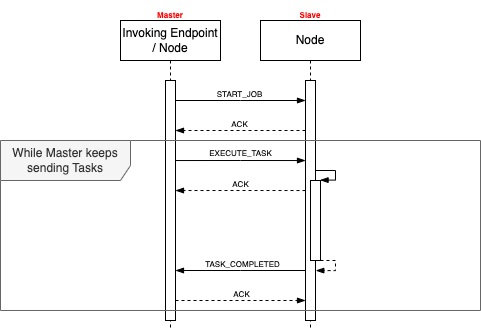
\includegraphics[scale=0.61]{document/chapters/chapter_6/images/p2p_messages.png}
    \caption{P2P messaging - Sequence Diagram}
    \label{fig:p2p_messages}
\end{figure}

\textbf{The Master sends a \textit{START\_JOB} message to the Slave}, possibly including data (which need to be sent only once) that will later be useful when executing the specific Tasks for that Job. Once the Slave has started said Job, t\textbf{he Master sends a \textbf{EXECUTE\_TASK} message}, \textbf{containing further data that}, combined with the Job's payload, \textbf{is used to perform a computation}. Upon receiving the EXECUTE\_TASK message the \textbf{Slave} sends an ACK to the Master and \textbf{enqueues the Task}, sending a \textbf{\textbf{TASK\_COMPLETED}} message (containing the result) to the Master \textbf{only when the task is actually completed}.

\textbf{This asynchronous organization allows the Master to send multiple Tasks to enqueue without waiting that the Slave has already completed its Tasks, speeding up the process}.
The Tasks submission and collection of results continues until all the Master's Tasks are completed and the P2P connection is terminated, removing the Job from the Slave.

\textbf{Using this Job/Task generalization, it is possible to construct various kinds of Grid Services}, starting from the MapReduce one.